\documentclass[11pt]{article}
\usepackage{homework}

\classname{361}
\homeworknum{4}



\begin{document}

% Environments

\newcommand{\state}[2]{\begin{statement}{#1} #2 \end{statement}}
\newcommand{\prob}[2]{\begin{problem}{#1} #2 \end{problem}}
\newcommand{\subprob}[1]{\begin{subproblem} #1 \end{subproblem}}
\newcommand{\sol}[1]{\begin{solution} #1 \end{solution}}
\newcommand{\fig}[2]{\begin{figure} \centering #2  \label{#1} \end{figure}}

\newcommand{\makebib}{
	\vfill
	\color{black}
	\nocite{*}
	\bibliography{references}{}
	\bibliographystyle{lucas_unsrt}
}
	

% Implication

\newcommand{\qwhere}{\quad \text{where} \quad}
\newcommand{\qimplies}{\quad \implies \quad}
\newcommand{\impliesq}{\implies \quad}



% Brackets

\newcommand{\paren}[1]{\left( #1 \right)}
\newcommand{\brac}[1]{\left[ #1 \right]}
\newcommand{\curly}[1]{\left\{ #1 \right\}}


% Greek

\newcommand{\alp}{\alpha}
\newcommand{\bet}{\beta}
\newcommand{\gam}{\gamma}
\newcommand{\del}{\delta}
\newcommand{\eps}{\epsilon}
\newcommand{\zet}{\zeta}
\newcommand{\tht}{\theta}
\newcommand{\kap}{\kappa}
\newcommand{\lam}{\lambda}
\newcommand{\sig}{\sigma}
\newcommand{\ups}{\upsilon}
\newcommand{\omg}{\omega}

\newcommand{\Gam}{\Gamma}
\newcommand{\Del}{\Delta}
\newcommand{\Tht}{\Theta}
\newcommand{\Lam}{\Lambda}
\newcommand{\Sig}{\Sigma}
\newcommand{\Omg}{\Omega}


% Text

\newcommand{\where}{\text{where }}

% Problem 1

\newcommand{\Hint}{H_\text{int}}
\newcommand{\ddcx}{\dd[3]{x}}
\newcommand{\psib}{\bar{\psi}}

\newcommand{\mh}{m_h}
\newcommand{\mmu}{m_\mu}
\newcommand{\me}{m_e}
\newcommand{\ma}{m_a}

\newcommand{\aexpt}{a_\text{expt.}}
\newcommand{\aQED}{a_\text{QED}}
\renewcommand{\GeV}{\giga\electronvolt}

\newcommand{\gamt}{\gam^5}


\state{LCR circuit}{ \label{1a}
	An electrical circuit consists of an inductance $L$, resistance $R$ and capacitance $C$ in series, driven by a voltage source $\Vt = \Vo \cos(\omg t)$.
}

\prob{
	Show that the charge $\qt$ on the capacitor satisfies the equation
	\eqn{ODE}{
		L \qdd + R \qd + \frac{q}{C} = \Vt,
	}
	and use it to define the complex susceptibility from
	\eqn{susceptibility}{
		\qomg = \chiomg \Vomg.
	}
	Show that the forced solution of this equation is
	\eq{
		\qt = \frac{\Vo \cos(\omg t - \phi)}{\sqrt{ (-\omg^2 L + 1 / C)^2 + (\omg R)^2 }},
	}
	where
	\eq{
		\tan(\phi) = \frac{\omg R}{\omg^2 L - 1 / C}.
	}
	\vfix
}

\sol{
	An example LCR circuit is shown in Fig.~\ref{LCR}.  We can use Kirchoff's loop rule to obtain the differential equation for this circuit.  Beginning from the bottom left corner of the circuit and moving clockwise, we have~\cite[pp.~849, 1007]{YF}
	\eq{
		0 = \Vt - I R - L \dv{I}{t} - \frac{q}{C},
	}
	where we have applied Ohm's law $\Vab = I R$, the potential difference across an inductor $\Vab = L \dv*{I}{t}$, and the definition of capacitance $C = q / \Vab$~\cite[pp.~782, 999]{YF}.  The current $\It = \dv*{\qt}{t}$ and charge $\qt$ are identical at all points in a series circuit.  Feeding in $I = \dv*{\qt}{t}$, this relation becomes
	\eq{
		\ans{ \Vt = L \qdd + R \qd + \frac{q}{C} }
	}
	as we wanted to show. \qed
	
	\begin{figure}[b]
		\centering
		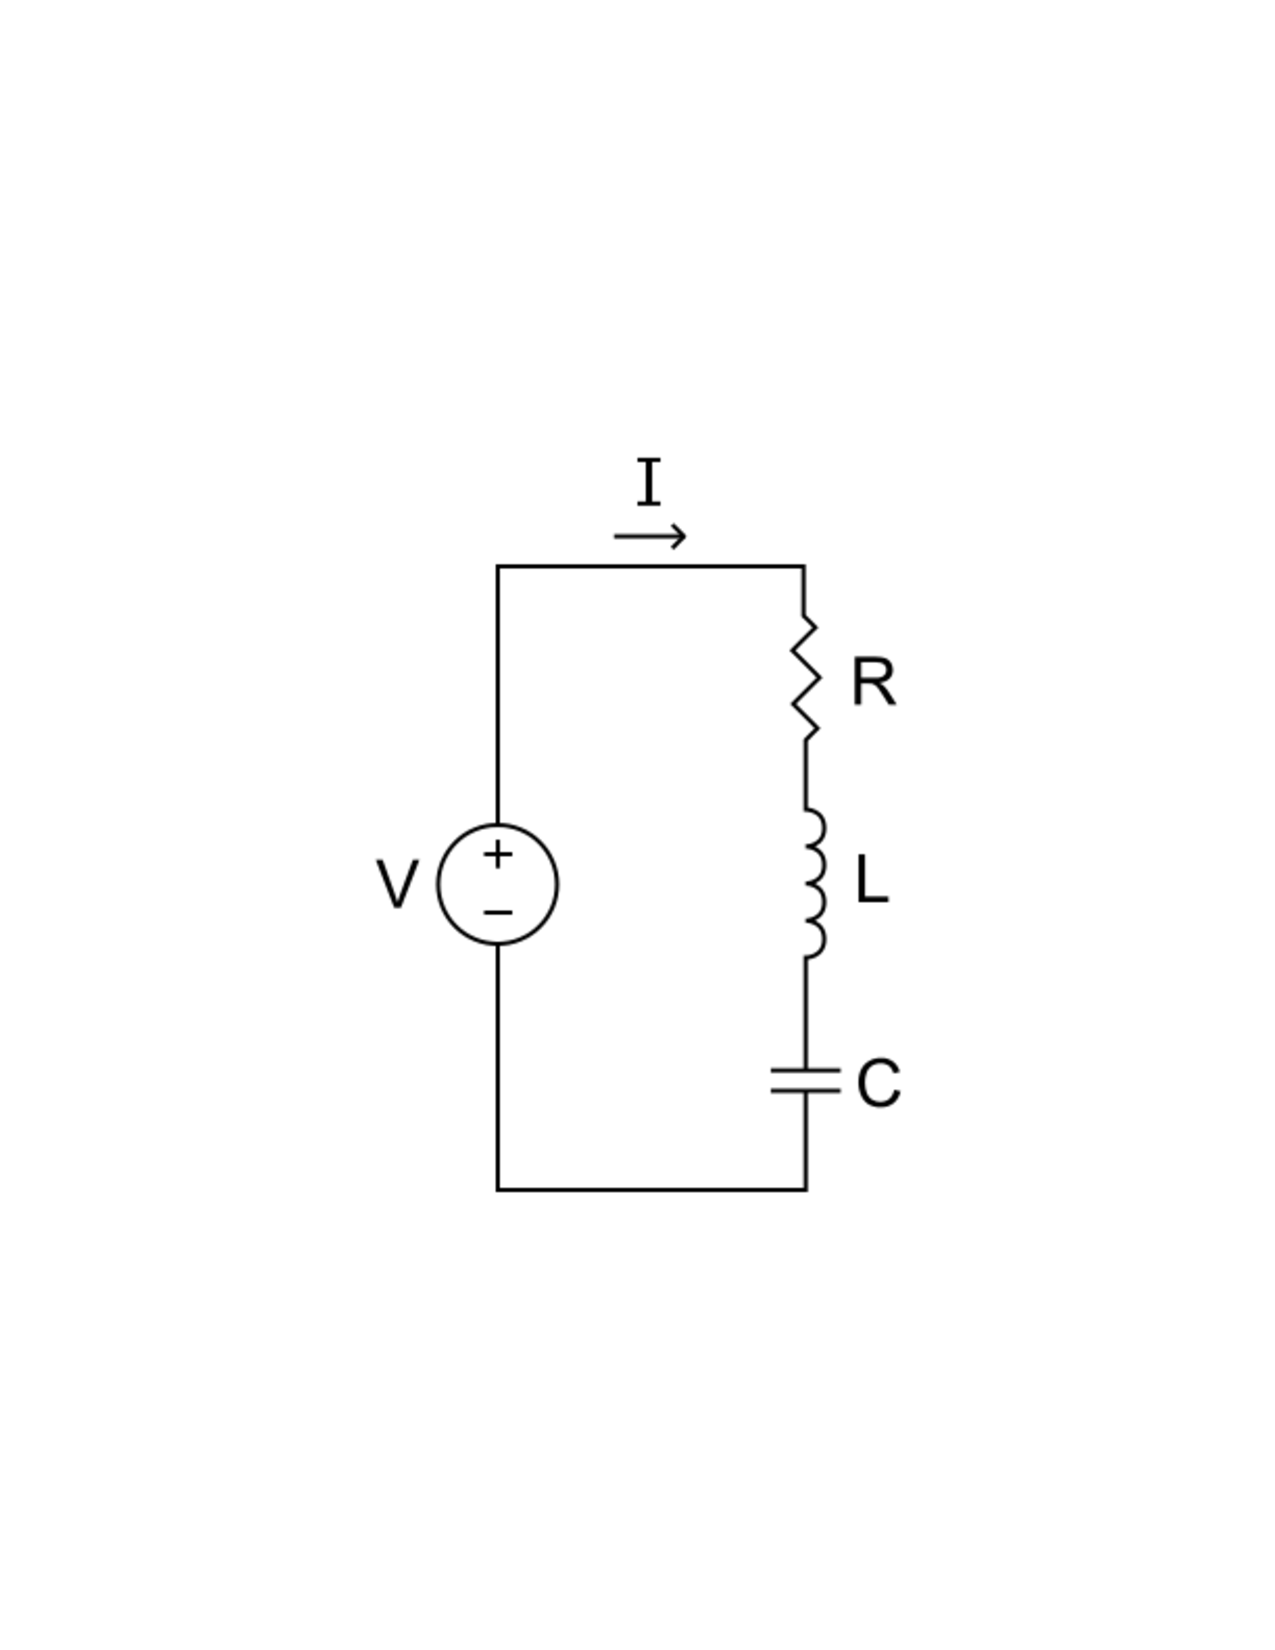
\includegraphics[width=0.15\textwidth,trim=6.25cm 7.75cm 6.25cm 7.75cm,clip]{RLC}
		\caption{An LCR series circuit~\cite{RLC}.}
		\label{LCR}
	\end{figure}
	
	Equation~\refeq{ODE} is an ODE representing forced damped motion of a mass-spring system.  Its solution can be written as the sum of the homogeneous solution, which dies out with time, and a particular solution~\cite[pp.~38, 40, 50--51]{Olmstead}.  Rewriting Eq.~\refeq{ODE} as
	\eq{
		\frac{\Vo}{L} \cos(\omg t) = \qdd + 2 p \qd + \omgo^2 q
	}
	where $p = R / 2 L$ and $\omgo^2 = 1 / L C$, the ansatz for the particular solution is
	\eq{
		\qt = \Ac \cos(\omg t) + \As \sin(\omg t).
	}
	Feeding this into the ODE and collecting terms yields
	\al{
		-\Ac \omg^2 + 2 p \As \omg + \omgo^2 \Ac &= \frac{\Vo}{L}, &
		-\As \omg^2 - 2 p \Ac \omg + \omgo^2 \As &= 0.
	}
	This system has the solutions~\cite[p.~51]{Olmstead}
	\aln{ \label{AcAs}
		\As &= \frac{2 p \omg \Vo / L}{4 p^2 \omg^2 + (\omgo^2 - \omg^2)^2}, &
		\Ac &= \frac{(\omg^2 - \omgo^2) \Vo / L}{4 p^2 \omg^2 + (\omgo^2 - \omg^2)^2}.
	}
	If we define
	\eqn{A}{
		A = \sqrt{\Ac^2 + \As^2}
	}
	and write
	\eq{
		\qt = A \paren{ \frac{\Ac}{A} \cos(\omg t) + \frac{\As}{A} \sin(\omg t), }
	}
	there exists an angle $\phi$ such that $\cos(\phi) = \Ac / A$, $\sin(\phi) = \As / A$, and $\tan(\phi) = \As / \Ac$.  Thus
	\eq{
		\qt = A [ \cos(\phi) \cos(\omg t) + \sin(\phi) \sin(\omg).
	}
	Using the identity
	\eq{
		\cos(\alp) \cos(\bet) + \sin(\alp) \sin(\bet) = \cos(\alp - \bet),
	}
	it follows that~\cite[pp.~39, 51]{Olmstead}
	\eq{
		\qt = A \cos(\omg t - \phi).
	}
	The amplitude $A$ is given by~\cite[p.~51]{Olmstead}
	\al{
		A &= \frac{C \Vo}{\sqrt{(\nu^2 - 1)^2 + 4 c^2 \nu^2}}, &
		\qwhere
		c &= \frac{R}{2 \sqrt{L / C}}, \quad
		\nu = \frac{\omg}{\omgo}.
	}
	Substituting back to the original quantities, this is
	\eq{
		A = \frac{C \Vo}{\sqrt{(\omg^2 / \omgo^2 - 1)^2 + (R^2 C / L) (\omg^2 / \omgo^2) }} \\
		= \frac{C \Vo}{\sqrt{(L C \omg^2 - 1)^2 + C^2s R^2 \omg^2 }} \\
		= \frac{\Vo}{\sqrt{ (-\omg^2 L + 1 / C)^2 + (\omg R)^2 }}.
	}
	Additionally, from $\tan(\phi) = \As / \Ac$,
	\eq{
		\tan(\phi) = \frac{2 p \omg}{\omg^2 - \omg0^2}
		= \frac{R \omg / L}{\omg^2 - 1 / L C}
		= \ans{ \frac{\omg R}{\omg^2 L - 1 / C}. }
	}
	Hence we have shown
	\eq{
		\ans{ \qt = \frac{\Vo \cos(\omg t - \phi)}{\sqrt{ (-\omg^2 L + 1 / C)^2 + (\omg R)^2 }} }
	}
	as desired. \qed
	
	Finally, the complex susceptibility is defined by
	\eq{
		\frac{\Vo \cos(\omg t - \phi)}{\sqrt{ (-\omg^2 L + 1 / C)^2 + (\omg R)^2 }} = \chiomg \Vo \cos(\omg t),
	}
	where we have substituted into Eq.~\refeq{susceptibility}.  This implies
	\eq{
		\ans{ \chiomg = \frac{\cos(\omg t - \phi)}{\cos(\omg t)} \frac{1}{\sqrt{ (-\omg^2 L + 1 / C)^2 + (\omg R)^2 }}. }
	}
	\vfix
}



\prob{
	Show that the mean rate of power dissipation is
	\eq{
		W = \frac{1}{2} \frac{ \omg \Vo^2 \sin(\phi)}{\sqrt{ (-\omg^2 L + 1 / C)^2 + (\omg R)^2 }}.
	}
}

\sol{
	The average power into a general AC circuit is~\cite[p.~1032]{YF}
	\eq{
		\Pav = \frac{1}{2} V I \sin(\phi),
	}
	where $I$ is the current amplitude, $V$ is the voltage amplitude, and $\phi$ is the phase angle determined in \ref{1a}~\cite[pp.~1028, 1032]{YF}.  Assuming the circuit is perfectly efficient, the average power into the circuit is equal to the average power it dissipates, so $W = \Pav$.  Clearly $V = \Vo$.  For I,
	\eq{
		\It = \dv{\qt}{t}
		= \dv{t}( \frac{\Vo \cos(\omg t - \phi)}{\sqrt{ (-\omg^2 L + 1 / C)^2 + (\omg R)^2 }} )
		= -\frac{\omg \Vo \sin(\omg t - \phi)}{\sqrt{ (-\omg^2 L + 1 / C)^2 + (\omg R)^2 }},
	}
	so
	\eq{
		I = \frac{\omg \Vo}{\sqrt{ (-\omg^2 L + 1 / C)^2 + (\omg R)^2 }}.
	}
	Thus
	\eq{
		W = \frac{1}{2} V I \sin(\phi) = \ans{ \frac{1}{2} \frac{ \omg \Vo^2 \sin(\phi)}{\sqrt{ (-\omg^2 L + 1 / C)^2 + (\omg R)^2 }} }
	}
	as we wanted to show. \qed
}



\prob{
	Sketch the real and imaginary parts of $\chi$ as a function of frequency, for the cases $Q \ll 1$, $Q \approx 1$, and $Q \gg 1$, where $Q = \sqrt{L / C} / R$ is the ``quality factor.''
	
	Where are the poles of $\chi$ in the complex $\omg$ plane?
}

\sol{
	\hl{How is it even complex?}
}






%\state{Landau theory of phase transitions}{
%	A ferroelectric crystal is one that supports a macroscopic polarization $P$, which usually arises because the underlying crystal structure does not have inversion symmetry.  However, as temperature or pressure is changed, the crystal may recover the inversion symmetry.  This can be modeled by Landau's theory of second order phase transitions, where we postulate a form for the free energy density (per unit volume)
%	\eqn{given2}{
%		\cF = \frac{1}{2} a P^2 + \frac{1}{4} b P^4 + \frac{1}{6} c P^6 + \cdots,
%	}
%	where the coefficient $a = \ao (T - \Tc)$ is temperature dependent and all the other coefficients are constant.  Although the polarization $P$ is of course a vector, we assume that it can point only in a symmetry direction of the crystal, and so it is replaced by a scalar.
%}

%\prob{
%	Assume that $b > 0$ and $c = 0$.  Use Eq.~\refeq{given2} to determine the form for the equilibrium $\PT$.
%}



%\prob{ \label{2c}
%	Including in $\cF$ the energy of the polarization coupled to an external electric field $E$, determine the dielectric susceptibility $\chi = \dv*{P}{E}$ both above and below the critical temperature.
%}



%\prob{
%	Sketch curves for $\PT$, $\chiinvT$, and $\chiT$.
%}



%\prob{
%	In a different material, the free energy is described by a similar form to Eq.~\refeq{given2}, but with $b < 0$ and $c > 0$.  By sketching $\cF$ at different temperatures, discuss the behavior of the equilibrium polarization and the linear susceptibility, contrasting the results with those found in \ref{2c}.
%}






%\state{Reflectivity of metals}{
%	The phase velocity of light in a conducting medium is the speed of light divided by the complex dielectric constant $\Nomg = \sqrt{\epsomg}$ where we may use for $\eps$ the Drude result
%	\eq{
%		\epsomg = 1 - \frac{\omgp^2}{\omg^2 + i \omg / \tau}.
%	}
%	In a good Drude metal, we have $1 / \tau \ll \omgp$.
%}

%\prob{
%	Sketch curves of
%	\begin{enumerate}
%		\item $\Re[\sigomg]$,
%		\item $\Re[\epsomg]$,
%		\item $\Im[1 / \epsomg]$.
%	\end{enumerate}
%}



%\prob{
%	Consider a light wave with the electric field polarized in the $x$ direction at normal incidence from the vacuum on a good Drude metal occupying the region $z > 0$.  In the vacuum ($z < 0$), the incident $\Eq$ and reflected $\Ew$ waves give rise to a field
%	\eq{
%		\Ex = \Eq e^{i \omg (z / c - t)} + \Ew e^{-i \omg (z / c + t)},
%	}
%	whereas in the medium, the electric field is
%	\eq{
%		\Ex = \Eo e^{i \omg [ \Nomg z / c - t ]}.
%	}
%	Matching the electric and magnetic fields on the boundary, show that
%	\al{
%		\Eo &= \Eq + \Ew, &
%		N \Eo &= \Eq - \Ew,
%	}
%	and hence show that the reflection coefficient satisfies
%	\eq{
%		R = \abs{\frac{\Ew}{\Eq}}^2
%		= \abs{\frac{1 - N}{1 + N}}^2.
%	}
%}



%\prob{
%	Using the Drude formula above, show that
%	\eq{
%		R \approx \begin{cases}
%			1 - 2 \sqrt{\dfrac{\omg}{2\pi \sigo}} & \omg \ll 1 / \tau, \\[3ex]
%			1 - \dfrac{2}{\omgp \tau} & 1 / \tau \ll \omg \ll \omgp, \\[3ex]
%			0 & \omgp \ll \omg,
%		\end{cases}
%	}
%	and sketch the reflectivity $\Romg$.
%}






%\state{Phonons}{
%	From Eq.~(5.8) construct $\Im[\chi]$ in the limit that $\gam \to 0$.  Use the Kramers--{\Kronig} relation to then reconstruct $\Re[\chi]$ from $\Im[\chi]$ in the same limit.
%}






%\state{Screened Coulomb interaction}{
%	Consider a nucleus of charge $Z$ producing a potential
%	\eq{
%		\Vextvq = -\frac{4\pi Z e^2}{q^2}.
%	}
%	Using the long-wavelength limit of the dielectric function, show that the screened potential satisfies
%	\eq{
%		\Vscrvqo = -\frac{2}{3} \Omg \EF,
%	}
%	where $\Omg$ is the volume of the unit cell and $\EF$ is the Fermi energy for $Z$ free electrons per unit cell.
%}






%\state{Peierls transition}{
%	By rewriting the term containing $\nkpq$ (replace $\vk + \vq \to -\vk'$ and then relabel $\vk'$ as $\vk$), show that the static density response function can be written
%	\eq{
%		\chiovqo = 2 \sumklkF \frac{1}{\epskpq - \epsk}.
%	}
%	In one dimension, make a linear approximation to the electronic dispersion near $\kF$, i.e.~$\epsk = \vF \abs{k}$, and consider the response for $q = 2 \kF + p$, where $p \ll 2 \kF$.  By considering terms in the sum over $k$ near $k \approx -\kF$, show that
%	\eq{
%		\chio(2 \kF + p) \approx \frac{1}{2\pi \vF} \ln\abs{ \frac{\kF}{p} }.
%	}
%	Explain why this result suggests that a one-dimensional metal will be unstable to a lattice distortion with wavevector $2 \kF$.
%}






%\state{Optical properties}{
%	Discuss why, at optical frequencies, glass is transparent and silver is shiny, while graphite appears black and powdered sugar is white.
%}





%\state{Metals and insulators}{
%	Explain the differences between a metal and an insulator.  Your discussion should include reference to single particle properties, screening of the Coulomb interaction, optical properties, and electrical and thermal properties.
%}


\makebib

\end{document}
